\section{Introductory Example}

\subsection{Dynamic dispatch in matrix functions}

Dynamic, i.e.\ late bound, dispatch allows for high performance
polyalgorithms with specialized code paths depending on matrix properties which
can only be inferred at runtime based on the specific values of the inputs. For
example, the matrix square root (\verb|sqrtm|) has two methods defined:

\begin{itemize}
	\item For symmetric (or Hermitian) matrices, where the answer can be
		computed by diagonalization,
	\item For general dense matrices, where the answer uses the more
		expensive (but also more general) Schur
		factorization~\cite{Higham2008}.
\end{itemize}
%
The latter method contains a run time check for symmetry and dispatches upon
the former if present. Thus as summarized in Figure~\ref{fig:sqrtm}, dynamic
dispatch allows the same performant kernel to be called even in situations
where the user does not know if a particular input matrix is symmetric, or even
that specialized algorithms for symmetric matrices exist.

\begin{figure}
	\centering
	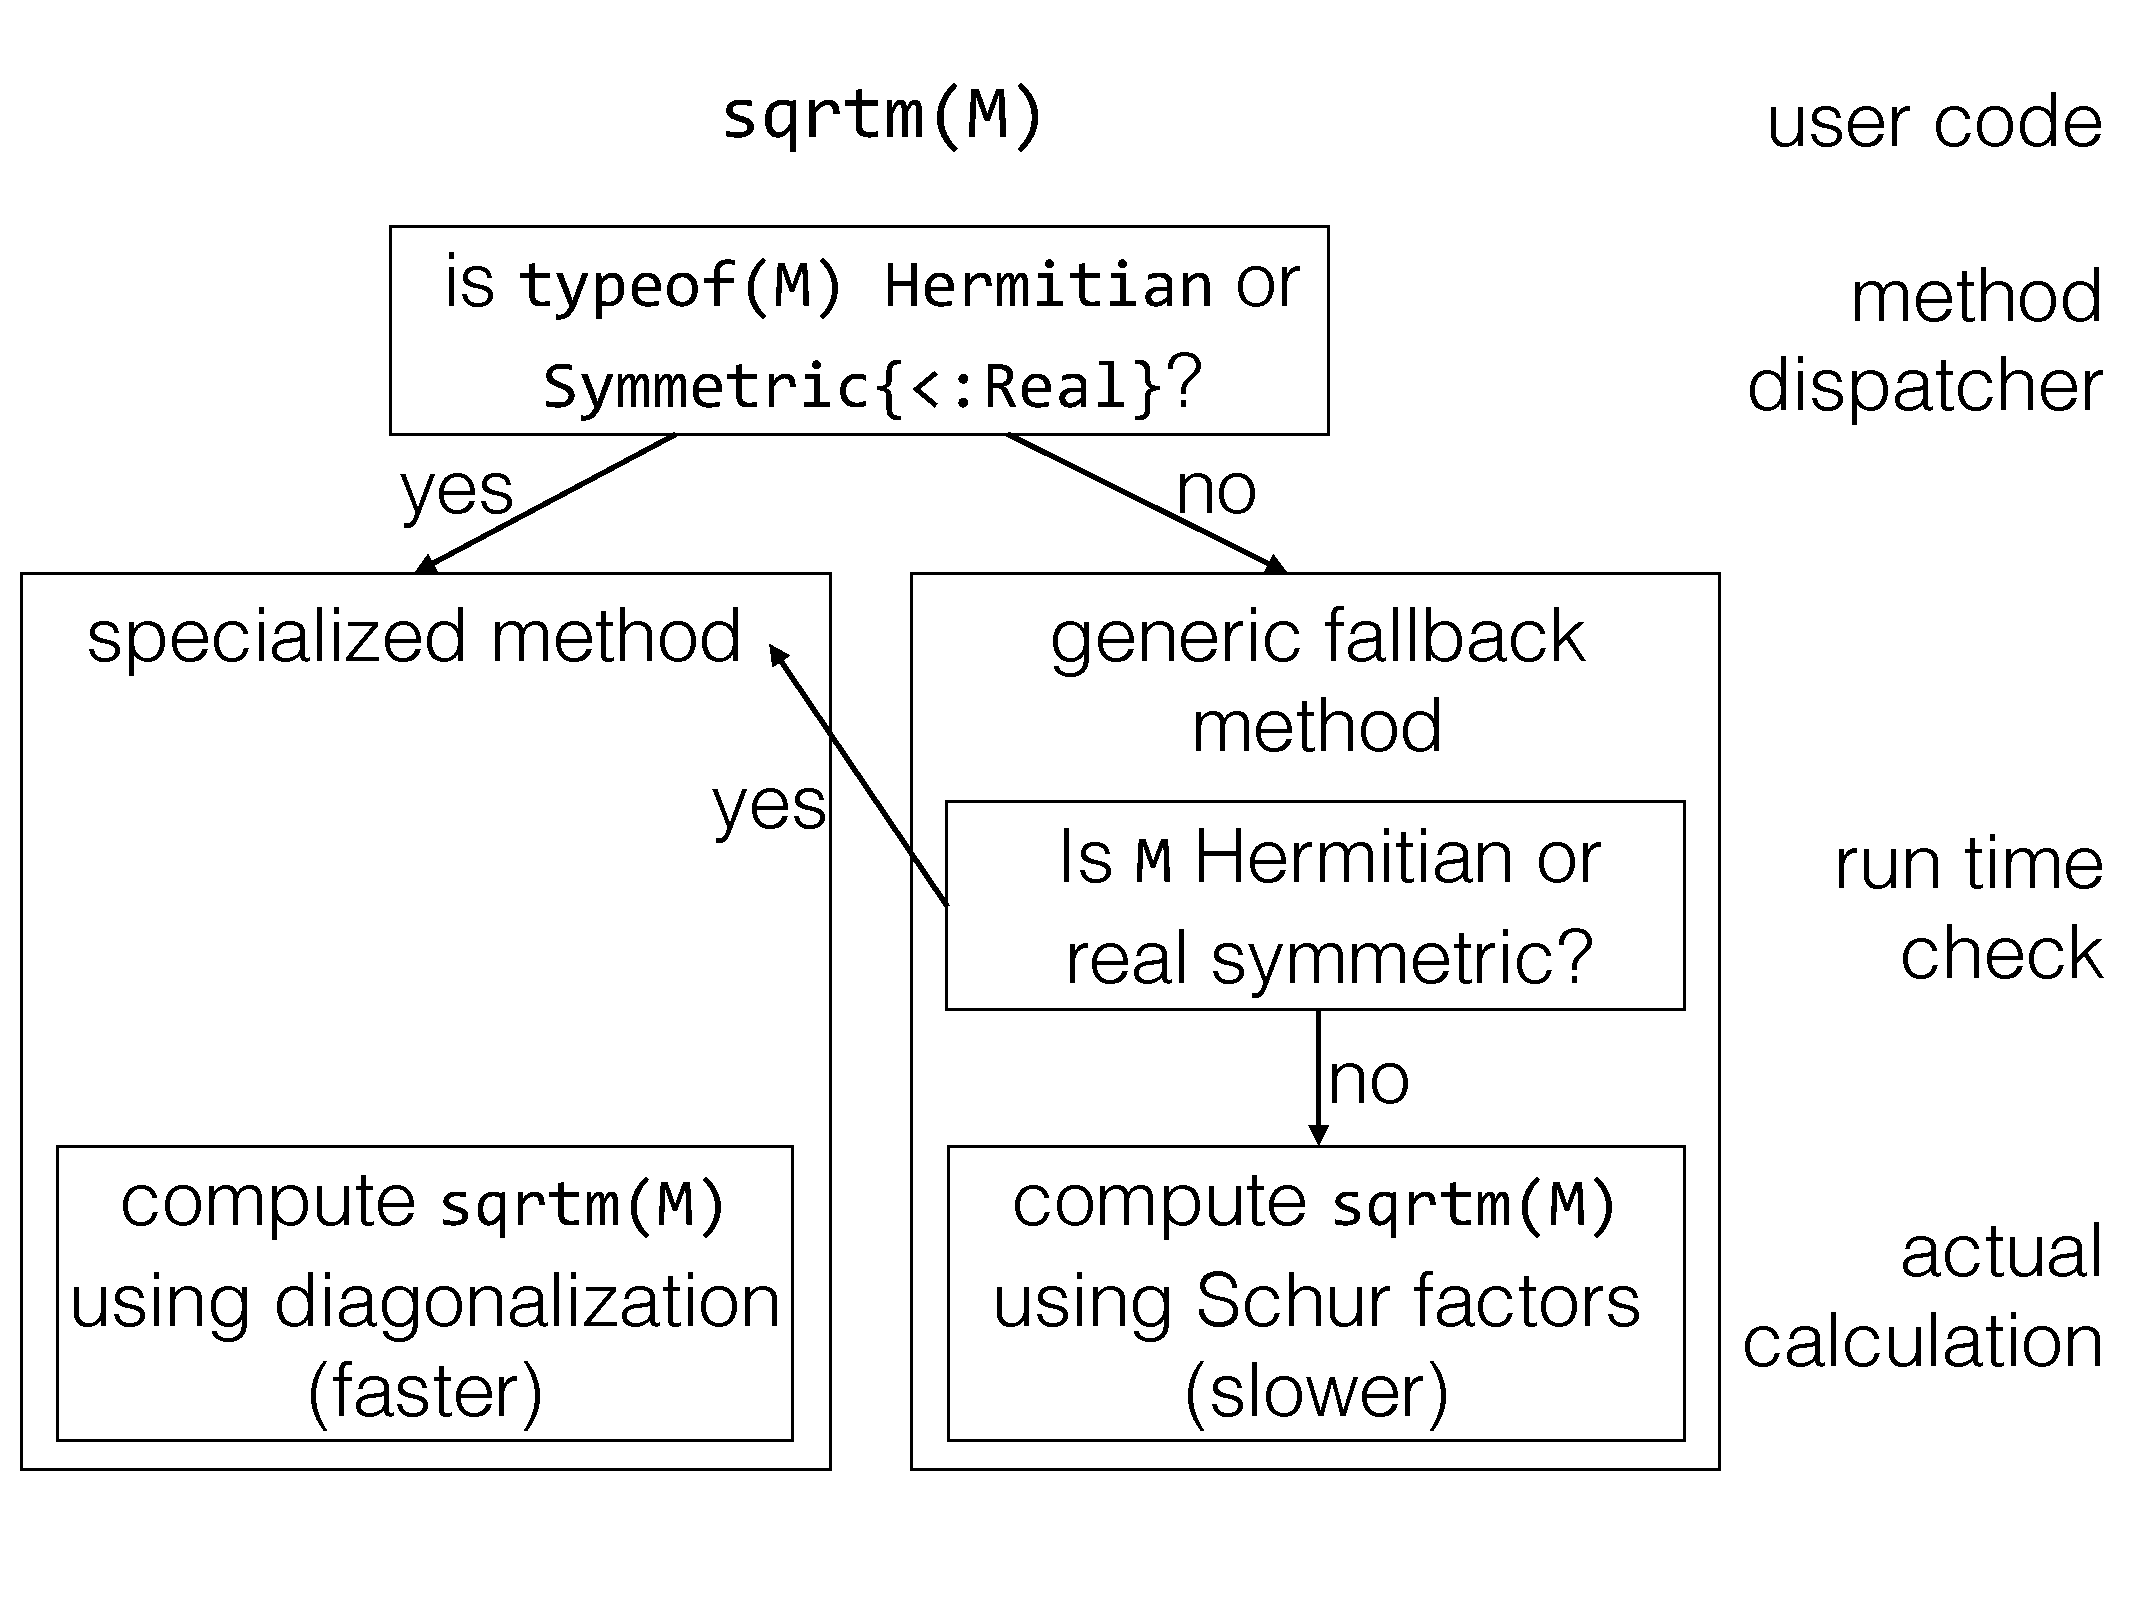
\includegraphics[width=\columnwidth]{fig-sqrtm}
	\caption{Dynamic dispatch and multimethods for the matrix square root
		function \texttt{sqrtm}, showing that the specialized algorithm
		can be run either from a static decision from the method
		dispatcher based on the input type, or a dynamic decision from
		a run-time check based on the value.}
	\label{fig:sqrtm}
\end{figure}




\subsection{Late binding increases expressiveness}

The examples in this section, while simple, illustrate the expressive power
afforded by the composition of extensible generic functions, polymorphic types,
dynamic multiple dispatch, and aggressive method specialization allowed by
just-in-time static analyses. Users are allowed to extend both the collection
of generic functions and the base type hierarchy in Julia, which further erodes
the distinction between user code and library code that is itself written in
Julia. We believe that such expressivity is useful for technical computing
applications, where it is not generally possible to predict the variety of
specialized computations that domain scientists, engineeers and mathematicians
require.

Some other languages also offer constructs for type polymorphism, like C++'s
expression templates and Fortress's generic functions, but these constructs are
only available at compile time, which restrict their expressiveness.
Furthermore, these languages usually require that all possible specialized
methods be generated at compile time, resulting in long compilation times which
are curtailed in practice with further restrictions on the generality of user
defined code. In contrast, the combination of dynamic multiple dispatch
semantics and on-demand method specialization in Julia allows users to write
highly generic code. Consider that the method definitions above each represent
an infinite family of methods. While user code in practice only uses a small,
finite subset of the possible methods, users have the luxury of choosing from
the entire universe encompassed by the generic function system.

